\documentclass[letterpaper]{article}
\usepackage[submission]{aaai25}
\usepackage{times}
\usepackage{helvet}
\usepackage{courier}
\usepackage[hyphens]{url}
\usepackage{graphicx}
\urlstyle{rm}
\def\UrlFont{\rm}
\usepackage{natbib}
\usepackage{caption}
\usepackage{booktabs}
\usepackage{amsmath}
\usepackage{amssymb}
\usepackage{xcolor}
\usepackage{multirow}
\usepackage{microtype}
\usepackage{placeins}   % \FloatBarrier
\usepackage{float}      % [H] placement option
\frenchspacing
\clubpenalty=10000
\widowpenalty=10000
\displaywidowpenalty=10000
\setlength{\pdfpagewidth}{8.5in}
\setlength{\pdfpageheight}{11in}

\renewcommand{\topfraction}{0.95}
\renewcommand{\textfraction}{0.05}
\renewcommand{\floatpagefraction}{0.85}
\renewcommand{\dbltopfraction}{0.95}
\renewcommand{\dblfloatpagefraction}{0.85}

\pdfinfo{
/TemplateVersion (2025.1)
}

\setcounter{secnumdepth}{0}

\title{Restoring the Image Does Not Restore Navigation:\\ Diagnosing Degradation-Robust Object-Goal Navigation as a Commitment Problem}

\author{Anonymous submission}
\affiliations{}
\makeatletter
\let\DRPN@old@maketitle\@maketitle

\def\@maketitle{%
  \DRPN@old@maketitle
  \par\vspace{-0.8em}

  \begin{minipage}{\textwidth}
    \centering

    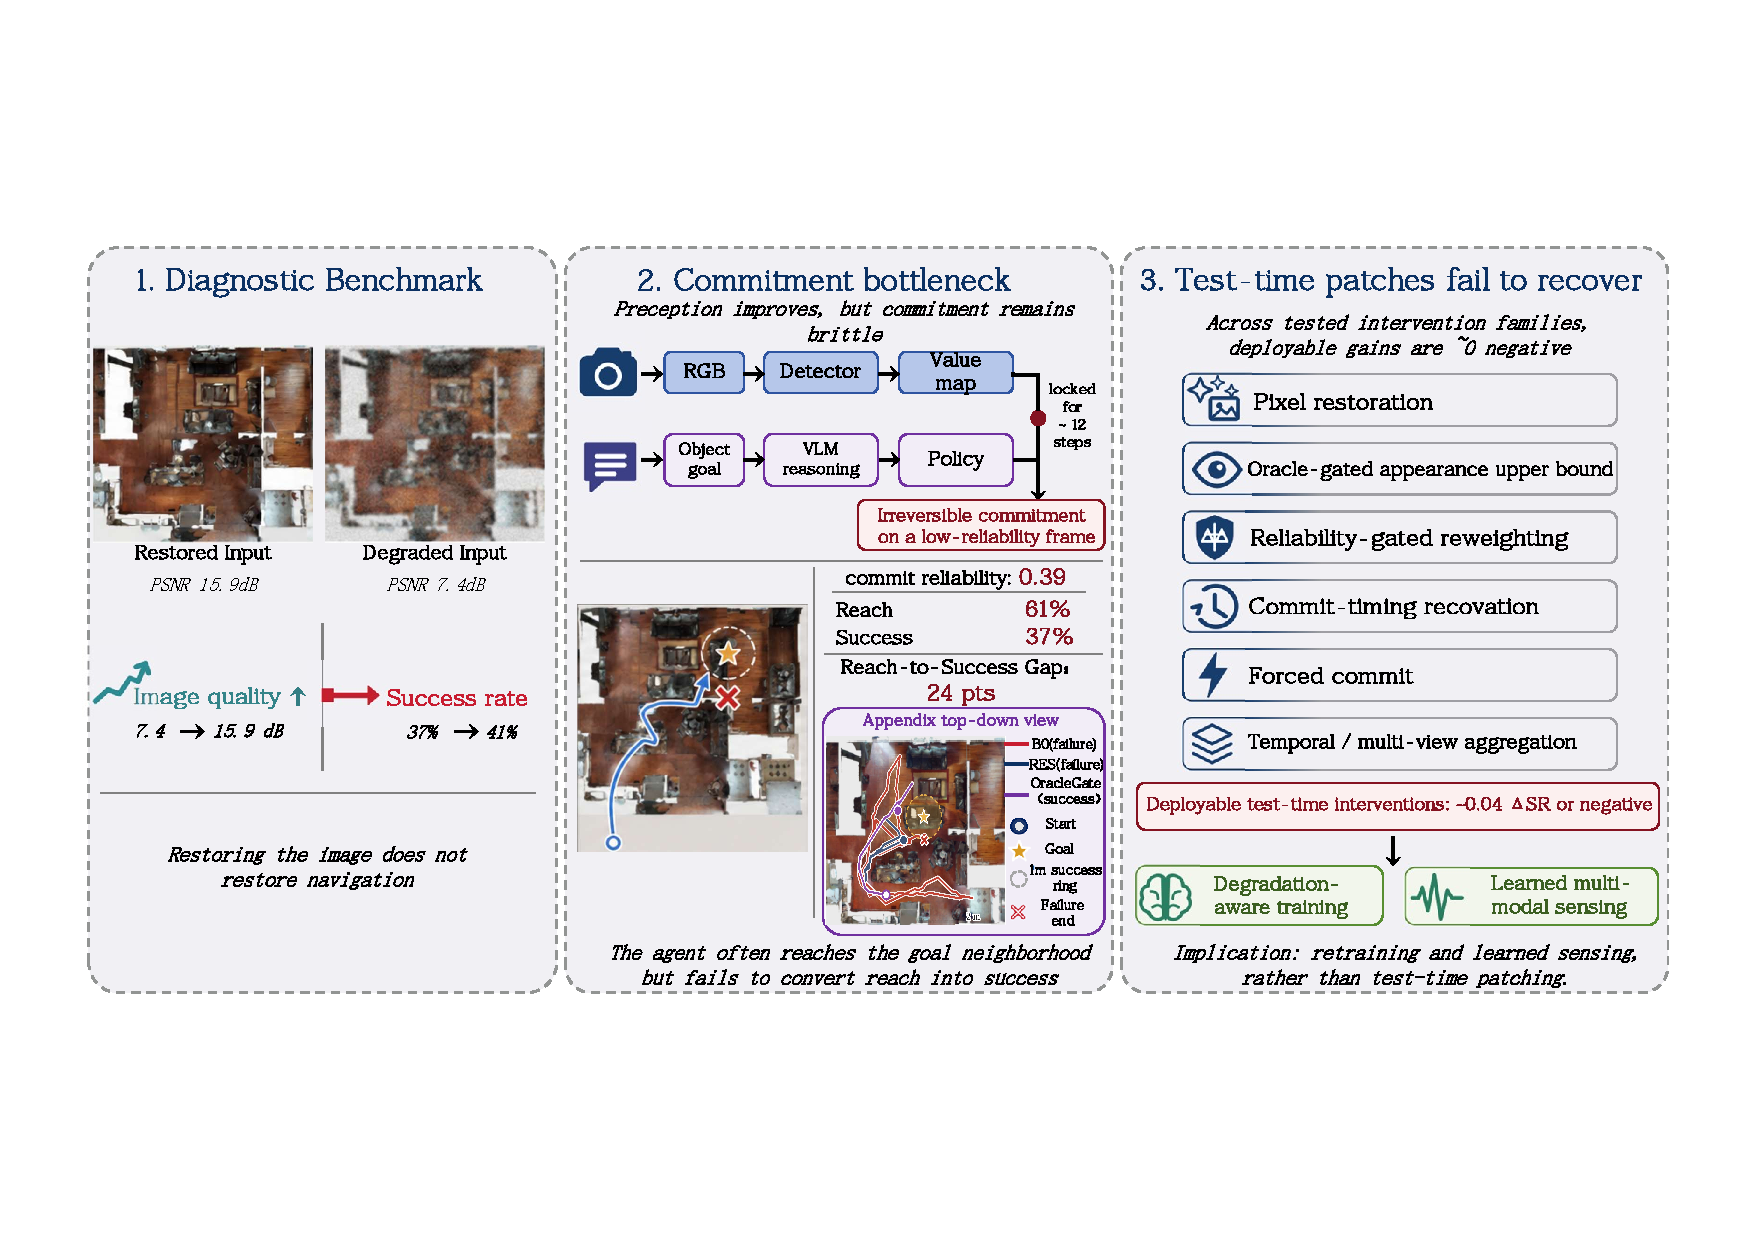
\includegraphics[
      width=1.0\textwidth,
      trim=3 3cm 0 4cm,
      clip
    ]{figures/motivation.pdf}

    \vspace{-0.4em}

    \captionof{figure}{
      \textbf{Restoring the image does not restore navigation.}
      \textbf{Left:} Restoration improves PSNR from $7.4$ to
      $15.9$\,dB, but success rises only from $37\%$ to $41\%$.
      \textbf{Middle:} Under low-light severity $4$, the agent reaches
      within $1$\,m in $61\%$ of episodes but succeeds in only $37\%$,
      revealing a $24$-point commitment gap.
      \textbf{Right:} Deployable test-time fixes yield only
      ${\sim}{+}0.04$ $\Delta$SR at best or negative gains, motivating
      degradation-aware training and learned multimodal sensing.
    }
    \label{fig:teaser}
  \end{minipage}

  \par\vspace{0.4em}
}
\makeatother

\begin{document}
\maketitle

\begin{abstract}
Zero-shot object-goal navigation agents driven by vision--language
models lose much of their success rate once the camera input is
corrupted by low light, haze, or motion, and a common remedy is to
restore the image before it reaches the policy. Through a controlled
study on InstructNav in Habitat--Matterport 3D ObjectNav, with a
same-seed paired protocol at $N{=}300$ and a blind per-step reliability
estimator, we show that this remedy targets the wrong layer.
Degradation does not stop the agent from acting; it corrupts the
quality of an irreversible commitment: the agent still reaches within
one metre of the goal in $61\%$ of episodes yet succeeds in only
$37\%$, and restoration that visibly repairs the image moves success
by a non-significant $+0.04$. A sweep over six causal families of
test-time interventions---pixel restoration with a per-frame appearance
upper bound, reliability-gated reweighting, commit-timing revocation,
forced commitment, temporal/multi-view aggregation, and a depth-based
multimodal probe---finds that every deployable family lands at
${\sim}0$ or significantly hurts success, evidence for a commitment
error that none of the probed test-time channels recovers.
The fingerprint survives a cross-corruption replication
(low-light, motion-blur, fog, Gaussian noise) on the same
InstructNav+Qwen2-VL-7B pipeline. These
results point the field away from test-time patches on frozen,
clean-trained agents, toward degradation-aware training and learned
multi-modal sensing. We release the benchmark, the paired protocol,
and all of the negative results.
\end{abstract}
\section{Introduction}

Object-goal navigation requires an agent to locate an instance of a target
category in an unknown environment, perceiving, deciding, and moving in a
closed loop \citep{batra2020objectnav}.  Recent zero-shot navigators delegate
the perceptual part of this loop to large vision--language models: a
panoramic observation is described in language, a heading is selected, and a
value map that scores candidate directions is updated at every step
\citep{long2024instructnav,yokoyama2024vlfm,zhou2023esc}. These methods perform
well on standard benchmarks, where the input is clean. In real deployments,
however, corridors are dimly lit, lenses fog up, and motion blurs the
image. Under these conditions, the same agents lose much of their success
rate: in our measurements, low light halves the success rate of a
representative zero-shot navigator on a held-out slice, and the paired
drop remains significant at $N{=}300$.

A natural remedy is to treat this as an image-quality issue and insert a
restoration front-end between the camera and the policy
\citep{guo2020zerodce,wu2023uretinex}, assuming that once the frame looks
clean  the navigator behaves as if the degradation were absent.
Whether this assumption holds has, to our knowledge, not been examined
directly for VLM-driven navigators. We find that it does not, and use a controlled
diagnosis to show \emph{why}. This is a diagnosis-and-benchmark paper: our
contribution is the measurement instrument and the resulting map of what
does not work, not a new agent.

\paragraph{A degradation-robust ObjectNav benchmark.}
We first build an evaluation substrate for this question: a degradation-robust
ObjectNav benchmark on a representative zero-shot backbone
(InstructNav~\citep{long2024instructnav}) in Habitat--Matterport~3D
\citep{ramakrishnan2021hm3d,yadav2023hm3dsem}. It applies structure-preserving
corruptions (low light, haze, motion blur, sensor noise) across severities,
fixes the same episodes across methods through a same-seed same-episode paired
protocol that supports McNemar tests, and equips the agent with a training-free
blind per-step reliability estimator. Every quantity below is measured on the
unmodified agent at the $N{=}300$ main-split scale, so the diagnosis does not
depend on any proposed fix. Sample size matters at this scale: between
$N{=}40$ and $N{=}150$ the measured per-condition restoration effect
\emph{changes sign}.

\paragraph{Degradation breaks commitments, not perception.}
Three observations emerge (Figure~\ref{fig:motivation}). First, degradation
reduces success: under low light the success rate falls by roughly half.
Second, the bottleneck is not appearance: a restoration step that raises image
fidelity by $8.4$\,dB PSNR leaves the success rate within seed noise, and a
per-frame oracle that picks the better of degraded and restored views does no
better than blanket restoration. Third, degradation does not change
\emph{whether} the agent acts. We call the moment the agent irreversibly
declares the target found---the detector's \texttt{found} flag flipping on a
single frame---a \emph{commitment}; degradation modestly lowers the commit rate
(from $93\%$ on clean to $89\%$ on low-light) and leaves
pure-exploration failures near  clean level, but corrupts the
\emph{quality} of these irreversible commitments. Decomposing the outcome as
$\text{SR}=\text{reachability}-\text{commit/stop loss}$, the agent walks within
one metre of the goal in $61\%$ of episodes yet succeeds in only $37\%$; it
commits at a frame reliability of $0.39$ versus $0.88$ on clean input, only
$42\%$ of its commitments lead to success, and once committed it rarely
recovers. The agent does not fail because it cannot see; it fails because
it makes an irreversible decision on a single unreliable frame and cannot
revoke it.

\paragraph{Negative results that localize the bottleneck.}
The diagnosis predicts that perception-layer fixes should not help, and we
confirm this at $N{=}300$: blanket restoration moves SR by only $+0.04$
(McNemar $p{=}0.18$), and even a non-deployable per-frame appearance
oracle caps at $+0.057$. A sweep across six causal families (appearance,
where-to-go, commit timing, forced commitment, temporal and multi-view
aggregation, and a depth-based cross-modal verifier) finds that every
\emph{deployable} family either lands at a non-significant ${\sim}0$ or
\emph{significantly hurts} success (Table~\ref{tab:sweep}), indicating a
commitment error that none of the probed test-time channels recovers.

\paragraph{Contributions.}
\begin{itemize}
\item \textbf{Benchmark.} A degradation-robust ObjectNav benchmark on a
  zero-shot VLM backbone: structure-preserving corruptions across
  severities, a same-seed paired protocol with McNemar exact tests and
  bootstrap CIs, and a training-free blind per-step reliability estimator.
\item \textbf{Diagnosis.} A method-independent mechanism analysis at
  $N{=}300$ that reframes degradation-induced failure as irreversible,
  low-reliability commitments, quantified by a reachability/commit-loss
  decomposition.
\item \textbf{Negative results.} A sweep of six causal intervention
  families in which every deployable family caps at zero or backfires
  ($p{<}0.05$), while the non-deployable per-frame appearance oracle caps
  at $+0.057$.
\item \textbf{Replication.} A cross-corruption replication (low-light,
  motion-blur, fog, Gaussian noise) reproducing the same non-significant
  fingerprint ($|\Delta\text{SR}|{\leq}0.05$, sign-flipping across
  cells), with every setting and seed released.
\end{itemize}

\FloatBarrier
\begin{figure*}[!t]
\centering
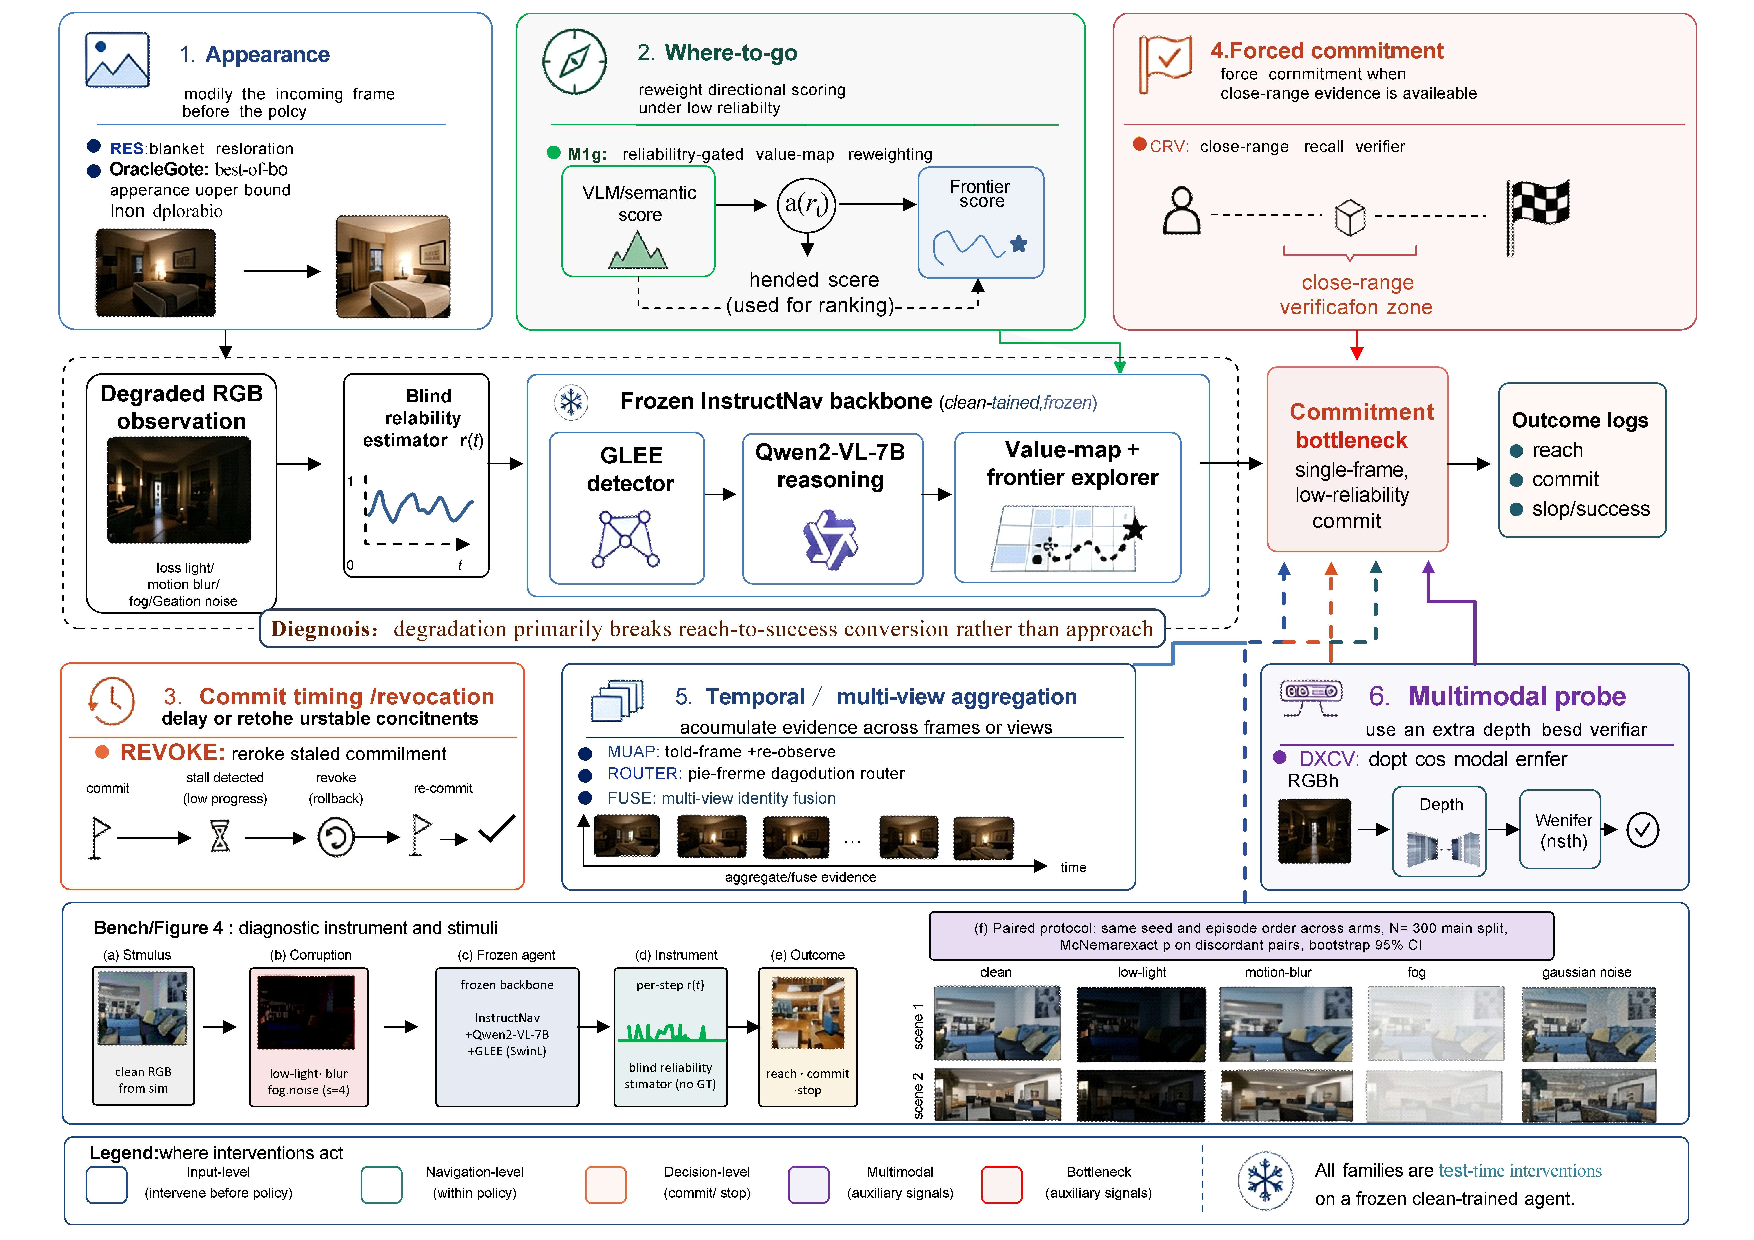
\includegraphics[width=0.88\textwidth]{figures/method.pdf}
\caption{
\textbf{From diagnosis to candidate interventions.}
A degraded RGB observation is passed through a blind per-step
reliability estimator and a frozen InstructNav backbone (GLEE,
Qwen2-VL-7B, and a value-map frontier explorer), whose outcome logs
localize failure to a \emph{commitment bottleneck}
(Sec.~\ref{sec:motivation}): degradation primarily breaks
reach-to-success conversion rather than approach.
The six surrounding panels instantiate the intervention families tested
in this paper: \textbf{(1)} appearance modification (RES, OracleGate),
\textbf{(2)} reliability-gated where-to-go reweighting,
\textbf{(3)} commit timing / revocation,
\textbf{(4)} forced commitment,
\textbf{(5)} temporal / multi-view aggregation, and
\textbf{(6)} a depth-based multimodal probe.
The bottom strip summarizes the benchmark substrate and paired protocol:
structure-preserving corruptions, a frozen clean-trained backbone, and
same-seed same-episode paired comparisons with McNemar exact tests and
bootstrap $95\%$ CIs.
}
\label{fig:method}
\end{figure*}

\section{Related Work}

\paragraph{Zero-shot object navigation with foundation models.}
Object-goal navigation \citep{batra2020objectnav} and vision-and-language
navigation \citep{anderson2018r2r,krantz2020vlnce,khanna2024goat} are
typically learned with reinforcement or imitation \citep{wijmans2020ddppo,
ramrakhya2023pirlnav}, which generalizes poorly to unseen distributions.
Zero-shot systems instead build on foundation models. One family
guides frontier exploration with language priors
\citep{chaplot2020semexp,zhou2023esc,yu2023l3mvn}; another fuses
open-vocabulary detectors into a value map for goal reasoning
\citep{yokoyama2024vlfm,gadre2023cow}; a third lets a VLM read a panoramic
observation and emit a heading \citep{zhou2024navgpt,
long2024instructnav}. We build on InstructNav \citep{long2024instructnav},
an agent that couples a VLM, an open-vocabulary detector
\citep{wu2024glee}, and a value-map frontier explorer. These works assume
clean observations; we instead study, on the same backbone, \emph{where}
such an agent breaks when its input is degraded.

\paragraph{Robustness of embodied agents to visual corruption.}
RobustNav \citep{chattopadhyay2021robustnav} first benchmarked navigation
under visual and dynamics corruptions and reported large drops, motivating
task-oriented data augmentation \citep{maksymets2021thda} and domain
adaptation. A common alternative is to restore the input before it reaches
the policy via low-light enhancement \citep{guo2020zerodce,wu2023uretinex}
or denoising, which operate at the pixel layer and aim to recover clean
appearance. We show that, for a VLM-driven navigator, restoring appearance
does not restore navigation: an $8.4$\,dB PSNR gain leaves SR within seed
noise, and a per-frame oracle that always picks the better-looking view
does no better. Our benchmark exposes this gap, with a paired protocol and
severity sweeps in the style of corruption robustness benchmarks
\citep{hendrycks2019benchmarking}.

\paragraph{Uncertainty, commitment, and executive control.}
Knowing when a model should not be trusted is central to safe autonomy
\citep{abdar2021uncertainty}; blind image-quality assessment estimates
degradation without a reference \citep{su2020blindly} and active perception
decides where to look to reduce uncertainty
\citep{ramakrishnan2021exploration}. A complementary direction studies the
\emph{executive} layer of zero-shot ObjectNav: \emph{when} to commit, stop,
and recover. We use a training-free per-step reliability estimate purely as
a \emph{measurement instrument}, and evaluate deployable commitment-timing
and temporal/multi-view aggregation interventions head-on; each leaves
success unchanged or lowers it on a frozen, clean-trained backbone
(Table~\ref{tab:sweep}).

\begin{figure*}[!t]
\centering
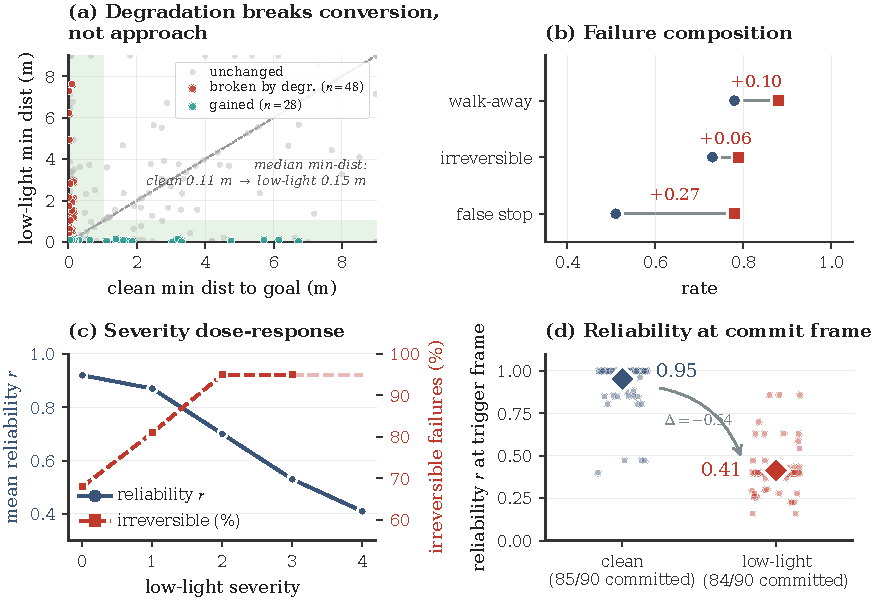
\includegraphics[width=0.88\textwidth]{figures/fig_motivation.pdf}
\caption{\textbf{Method-independent motivation study (baseline InstructNav).}
\textbf{(a)}~Paired min-distance, clean vs.\ low-light severity~$4$ (same
$300$ episodes): approach geometry barely moves (median $0.11\to0.15$\,m)
yet $48$ episodes flip to failure---degradation breaks \emph{conversion},
not approach. \textbf{(b)}~M2 ($n{=}90$): failures shift toward walk-aways
and irreversible failures. \textbf{(c)}~M3: severity lowers reliability;
the irreversible fraction saturates. \textbf{(d)}~M4: the deciding
commitment fires on a single low-$r$ frame (mean $0.95{\to}0.41$).}
\label{fig:motivation}
\end{figure*}
\begin{figure*}[t]
\centering
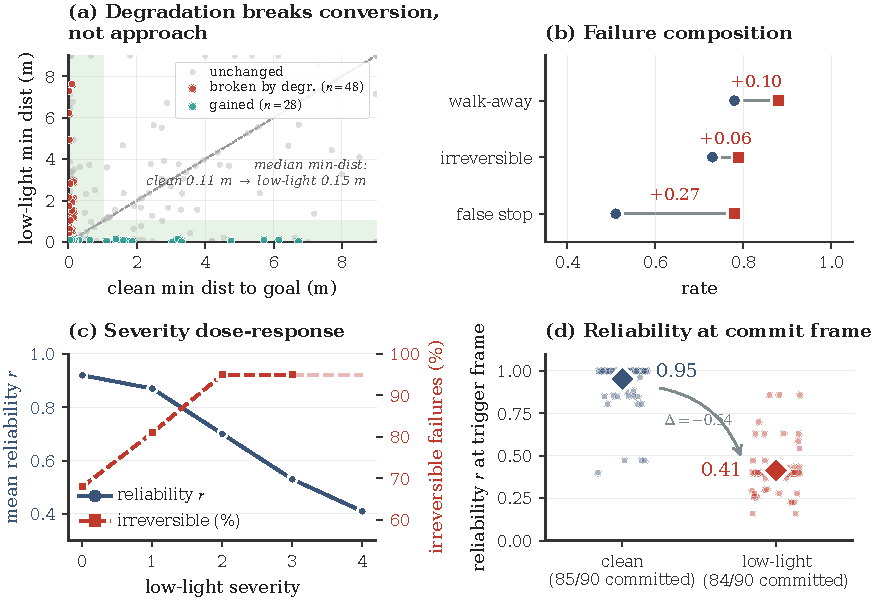
\includegraphics[width=\textwidth]{figures/fig_motivation.pdf}
\caption{\textbf{Method-independent motivation study (baseline InstructNav).}
\textbf{(a)}~Per-episode paired minimum distance to goal on the \emph{same}
$300$ episodes run clean and under low-light~s4: the approach geometry
barely moves (median min-dist $0.11\to0.15$\,m) yet $48$ episodes flip to
failure (red)---degradation breaks the reach-to-success \emph{conversion},
not the approach.
\textbf{(b)}~M2 ($n{=}90$): degradation shifts failures toward walk-aways and
irreversible failures, and false stops nearly double (walk-away and
irreversible: fraction of failed episodes; false stop: fraction of executed
stops that are false positives).
\textbf{(c)}~M3: as severity rises, mean reliability falls and the irreversible
fraction saturates at $95\%$.
\textbf{(d)}~M4: the deciding commitment fires on a single low-$r$ frame (mean
$r$ drops $0.95{\to}0.41$); once committed the agent stays locked for
${\sim}21$ steps. Coloured dots in (d) jitter the underlying per-commit $r$
distribution; diamonds are the means. $N$ counts episodes in which a commit
fired ($85$ and $84$ of the $90$ per condition; the remainder never
committed).}
\label{fig:motivation}
\end{figure*}

\section{Why Navigation Fails Under Degradation}
\label{sec:motivation}

A single episode previews the phenomenon this section quantifies. Asked to
find a toilet under low light, the baseline agent navigates to within
$0.02$\,m of it, never declares it found, wanders off, and the episode ends
in failure (Figure~\ref{fig:case-studies}c). The agent saw enough to get
there; what failed was the decision to stop. This section shows that the
pattern is systematic.

We analyze how visual degradation causes a zero-shot
navigator to fail. Every quantity is measured on the unmodified backbone, so
that the analysis does not depend on any component of our method. We organize
the study as five questions (M0--M4): whether degradation hurts at all (M0),
whether the cause is appearance (M1), what failures look like (M2), whether
reliability is informative about commitments (M3), and what triggers a
commitment (M4).

\paragraph{Setup.}
We run InstructNav on HM3D ObjectNav \texttt{val\_mini} pooled over seeds
$\{0,1,2\}$ ($n{=}90$, bootstrap $95\%$ CIs, $B{=}5000$). The primary
degradation is low-light at severity~$4$, drawn from a $13$-type
ImageNet-C-style suite \citep{hendrycks2019benchmarking}. The $n{=}90$
study below establishes the qualitative chain; the Experiments section
re-measures decisive quantities at $N{=}300$.

\paragraph{M0--M1: Degradation hurts, but appearance is not the lever.}
Low-light lowers SR from $0.433$ (CI $[0.333, 0.533]$) to $0.222$ ($[0.144,
0.311]$) at $n{=}90$; the paired drop is $-0.211$ with CI $[-0.322, -0.100]$,
excluding zero. Motion-blur gives $-0.056$ with CI
$[-0.167, +0.056]$ and does not exclude zero, so we use low-light as the
primary condition. Figure~\ref{fig:motivation}a shows \emph{where} the drop
lives at the paired $N{=}300$ scale: the per-episode minimum distance to
the goal is nearly unchanged (median $0.11\to0.15$\,m)---the agent still
gets to the goal---yet $48$ episodes flip to failure. Adding a test-time
restoration arm raises PSNR on
low-light from $7.4$ to $15.9$\,dB ($+8.4$\,dB) yet SR moves only $0.233
\to 0.300$, inside the $\pm0.10$ seed-noise band: making the image look
clean does not make the agent navigate.

\paragraph{M2: Failures are irreversible commitments.}
To characterize the failures, we distinguish \emph{walk-away} failures (the
agent ends far from a reachable goal and never returns) from \emph{false
stops} (premature, false-positive stops). A walk-away
is \emph{irreversible} when the trajectory was once closer to the goal but then
moved away and never came back. Degradation shifts the composition of failures
toward walk-aways: among failed episodes, the walk-away fraction rises from
$78\%$ on clean input to $88\%$ under low-light, and the irreversible fraction
from $73\%$ to $79\%$ (Figure~\ref{fig:motivation}b). The false-stop rate---the
fraction of executed stops that are false positives---rises in parallel, from
$0.51$ to $0.78$. Moreover, the reliability at the turning point $t^\star$,
where $d_t$ switches from decreasing to increasing, drops from $0.93$ on clean
input to $0.40$. The failures are thus not a matter of insufficient
exploration; they are early, confident commitments made when perception is
untrustworthy.

\paragraph{M3--M4: Reliability is informative; a single low-$r$ frame triggers the commitment.}
The reliability estimate carries a usable signal. On clean input, bucketing
commitments by $r$ shows net geodesic progress over the next five steps
rising monotonically with $r$ ($0.133/0.154/0.245$ for low/mid/high), and
across severities $0$--$4$ the mean $r$ falls monotonically
($0.92{\to}0.87{\to}0.70{\to}0.53{\to}0.41$) while the irreversible
fraction saturates at $95\%$ by severity~$3$ (Figure~\ref{fig:motivation}c).
The commitment itself is a single-frame event: the detector's
\texttt{found} flag flips on one frame, not after temporal consensus.
Across conditions, the $r$ of that triggering frame falls from $0.95$ on
clean to $0.41$ under low-light ($85$ and $84$ of the $90$ episodes per
condition committed at least once), and once made the
commitment persists for ${\sim}21$ steps (Figure~\ref{fig:motivation}d).
The entry point of the failure is an irreversible decision on one
unreliable frame.

\paragraph{M5: A reachability/commit-loss decomposition at the $N{=}300$ scale.}
The $M$-study above uses $n{=}90$; we now confirm the mechanism at the
$N{=}300$ main-split scale, where the baseline success rate is $0.36$ rather
than the $0.22$ of \texttt{val\_mini}. We decompose the outcome as
$\text{SR} = \text{reachability} - \text{commit/stop loss}$, where reachability
is the fraction of episodes whose trajectory passes within $1.0$\,m of the goal
(an upper bound achievable by a perfect stop policy on the \emph{actual}
trajectory, requiring no re-run; the threshold is calibrated from the $p_{90}$
stopping distance of clean successes, $0.15$\,m). On low-light at severity~$4$,
the baseline reaches within $1.0$\,m in $62.3\%$ of episodes but succeeds in
only $35.8\%$, a commit/stop loss of $26.5$ points: in one episode out of four
the agent passes the goal and fails to convert. Crucially, degradation does not
suppress \emph{action}: the commit rate is $93\%$ under low-light versus $94\%$
on clean input, and the pure-exploration-failure rate is ${\sim}6\%$ at both
ends. What collapses is commitment \emph{quality}: the reliability at the
committing frame falls from $0.95$ to $0.39$, the false-commit rate rises from
$55\%$ to $76\%$, only $40\%$ of commitments lead to success, and the agent
stays locked for ${\sim}12$ steps (${\sim}21$ in the $n{=}90$ study; the lock
is shorter on the easier main split but present at both scales). The same decomposition holds for
Gaussian noise (reachability ${\sim}0.59$, the loss again dominant), so the
pattern is not specific to low light.

\paragraph{Summary.}
The observations form a consistent chain: degradation does not blind the
agent and does not stop it from acting; it leads the agent to stake
irreversible heading and stop commitments on single, low-reliability
frames, so the resulting loss sits in the reach-to-success conversion
rather than in perception or exploration. The diagnosis predicts that
interventions on appearance or on where-to-go should not move success,
because they never touch the commitment conversion. The Method section
turns this into candidate interventions; the Experiments section confirms
the prediction across a six-family sweep in which no deployable arm moves
success and several lower it.

\FloatBarrier
\section{From Diagnosis to Candidate Interventions}
\label{sec:method}

The diagnosis specifies both \emph{what} fails (the quality of irreversible
commitments) and \emph{when} (when the committing frame is unreliable), and
makes a falsifiable prediction: interventions on image appearance or on
where-to-go should not move success, because the loss lives in the
reach-to-success conversion. To test this prediction we construct the most
natural candidate interventions the diagnosis suggests, spanning the pixel,
perception, and decision layers. A per-frame appearance oracle upper-bounds
per-frame arbitration over appearance. The instrument behind the test
(Figure~\ref{fig:pipeline}, Appendix) pairs the same frozen backbone on
clean and degraded versions of identical episodes.

\subsection{Per-Step Reliability Estimation}

We map each RGB frame to a scalar reliability $r\in[0,1]$ using a blind
detector bank that needs no reference frame or training. We combine cues
that respond to structure-preserving corruptions: mean luma for darkness,
global contrast and std.\ deviation for a haze veil, Laplacian energy for
blur, a dark-channel statistic for fog, and a noise estimate for sensor
noise. Each cue is calibrated once on a probe set so clean frames score
$r{\approx}1$ and corruptions lower $r$ monotonically
(Figure~\ref{fig:calibration}): clean $1.00$, low-light $0.65$,
motion-blur
$0.47$, fog $0.36$, Gaussian noise $0.20$. Throughout, $r$ serves as an
\emph{instrument}: it lets candidates gate on perceived trustworthiness,
but is not itself a contribution.

\begin{figure}[!t]
\centering
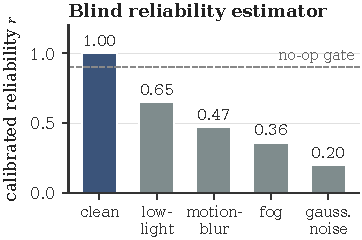
\includegraphics[width=0.52\columnwidth]{figures/fig_calibration.pdf}
\caption{\textbf{Blind reliability estimator $r$} on the calibration probe
set: clean frames score $r{\approx}1$; each structure-preserving
corruption lowers $r$ monotonically. Dashed line: the $r{=}0.9$ no-op
gate above which reliability-gated candidates reduce to the clean
baseline exactly.}
\label{fig:calibration}
\end{figure}

\subsection{Candidate 1 (Appearance): Blanket and Oracle-Gated Restoration}

The default remedy treats degradation as an image-quality problem and restores
the frame before the policy sees it. We include two variants. \emph{Blanket
restoration} (RES) always applies a low-light/denoising front-end. To upper-bound
\emph{any} test-time arbitration over appearance, we also define a \emph{per-frame
appearance oracle} (\textsc{OracleGate}) that, at every step, is allowed to pick
whichever of the degraded and restored views yields the better navigation
outcome. \textsc{OracleGate} is not deployable---it consults privileged
information---and it bounds any \emph{per-frame} router over restored
versus degraded appearance. If even \textsc{OracleGate} does not beat
blanket restoration, per-frame appearance arbitration has no headroom left
to exploit.

\subsection{Candidate 2 (Where-to-Go): Reliability-Gated Reweighting}

If appearance is not the lever, the diagnosis points to the decision layer.
A value-map navigator scores candidate headings by combining a
\emph{language--semantic term} $v_{\text{vlm+sem}}$ (which a corrupted frame
misleads) with a geometric frontier-coverage term $v_{\text{frontier}}$.
The reliability-gated reweighting candidate (R-Weight) takes a convex mixture
$v(a)=(1{-}\beta)v_{\text{vlm+sem}}(a)+\beta v_{\text{frontier}}(a)$, with
the mixing weight $\beta(r)$ gated by reliability: $\beta{=}0$ above
$\tau_{\text{gate}}{=}0.9$, and $\beta{=}\min(\beta_{\max},\alpha(1{-}r))$
below it ($\alpha{=}1$, $\beta_{\max}{=}0.6$), so on clean input R-Weight
reduces exactly to the backbone.

Together these candidates probe pixels (RES, OracleGate) and where-to-go
(R-Weight); \textsc{OracleGate} is an upper bound rather than a method, so
a collective failure to move success is a statement about \emph{where the
headroom is}, not about weak baselines. The Experiments section sweeps
four further families (commit timing/revocation, forced commitment,
temporal/multi-view aggregation, and a depth-based multimodal probe).

\FloatBarrier
\begin{figure*}[!t]
\centering
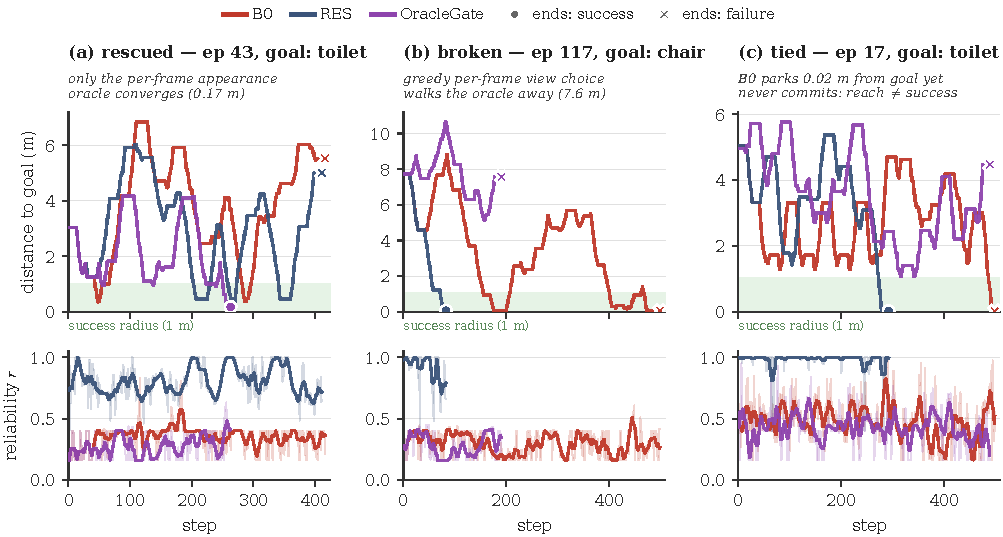
\includegraphics[width=0.68\textwidth]{figures/fig_case_studies.pdf}\\[2pt]
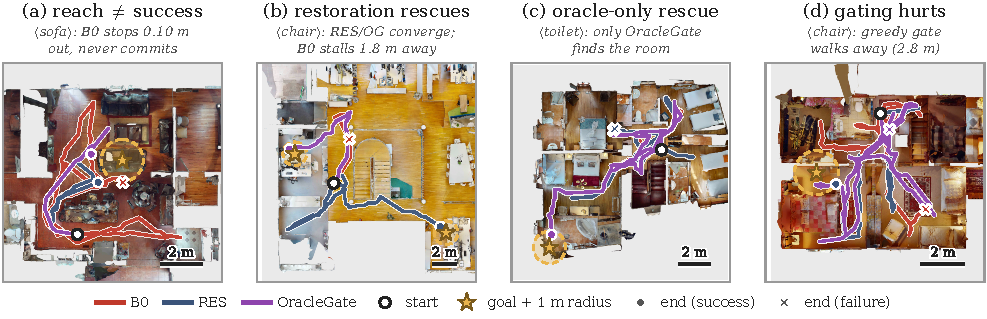
\includegraphics[width=0.68\textwidth]{figures/fig_trajectories.pdf}
\caption{\textbf{Episode-level views of the paired low-light cell.}
\emph{Top}: per-step distance to goal and reliability $r$ (B0, RES,
\textsc{OracleGate}, \emph{same} episode): a \emph{rescued}, a
\emph{broken}, and a \emph{tied} episode in which B0 touches $0.02$\,m
yet never commits---perception is restored, the decision is not.
\emph{Bottom}: top-down trajectories (stars: goal, $1$\,m radius).
Interventions reroute \emph{where} the agent goes far less than
\emph{whether} it commits.}
\label{fig:case-studies}
\label{fig:trajectories}
\end{figure*}

\begin{table*}[t]
\centering
\small
\setlength{\tabcolsep}{3.4pt}
\begin{tabular}{@{}lllcccccccc@{}}
\toprule
Family & Arm & What it does & SR$_{\text{B0}}$ & SR$_{\text{arm}}$ & $\Delta$SR & $\Delta$SPL & 95\% CI($\Delta$SR) & $p$ (McN.) & $N$ \\
\midrule
Appearance & RES & blanket restoration front-end & $0.370$ & $0.410$ & $+0.040$ & $+0.032$ & $[-0.013,+0.093]$ & $0.182$ & $300$ \\
Appearance UB & OracleGate$^{\ddagger}$ & per-frame best-of-two view & $0.370$ & $0.427$ & $\mathbf{+0.057}$ & $+0.025$ & $[+0.003,+0.110]$ & $\mathbf{0.043}$ & $300$ \\
Where-to-go & M1g & $r$-gated value-map reweight & $0.370$ & $0.410$ & $+0.040$ & $+0.012$ & $[-0.017,+0.097]$ & $0.201$ & $300$ \\
Commit timing & REVOKE & revoke stalled commitments & $0.380$ & $0.260$ & $\mathbf{-0.120}$ & $-0.020$ & $[-0.207,-0.040]$ & $\mathbf{0.006}$ & $150$ \\
Forced commit & CRV & close-range recall verifier & $0.380$ & $0.400$ & $+0.020$ & $+0.021$ & $[-0.053,+0.093]$ & $0.728$ & $150$ \\
Temporal & MUAP & hold-frames + re-observe & $0.380$ & $0.260$ & $\mathbf{-0.120}$ & $-0.039$ & $[-0.220,-0.020]$ & $\mathbf{0.022}$ & $150$ \\
Temporal & ROUTER & per-frame degradation router & $0.380$ & $0.393$ & $+0.013$ & $+0.031$ & $[-0.073,+0.100]$ & $0.875$ & $150$ \\
Multi-view & FUSE & multi-view identity fusion & $0.380$ & $0.367$ & $-0.013$ & $+0.032$ & $[-0.100,+0.073]$ & $0.878$ & $150$ \\
Multimodal probe & DXCV$^{\flat}$ & depth cross-modal veto & $0.380$ & $0.207$ & $\mathbf{-0.173}$ & $-0.057$ & $[-0.260,-0.087]$ & $\mathbf{{<}0.001}$ & $150$ \\
\bottomrule
\end{tabular}
\caption{\textbf{Intervention sweep across six causal families.} Paired protocol on low-light sev~$4$, seed~$0$, val split. The three top rows are scored at the $N{=}300$ main split; the six lower rows share a common $N{=}150$ subset with a single shared baseline, so all comparisons are on exactly the same episodes. Bold entries are significant at $p{<}0.05$ (McNemar exact). Every \emph{deployable} family either lands at a non-significant ${\sim}0$ or \emph{significantly hurts} success (REVOKE, MUAP, DXCV lower paired SR by $0.12$--$0.17$); the only arm clearing $p{<}0.05$ with a \emph{positive} $\Delta$SR is the non-deployable per-frame appearance upper bound, which caps at $+0.057$. Confidence intervals are $B{=}5000$ bootstrap over paired episode differences. $^{\ddagger}$non-deployable oracle. $^{\flat}$train-free depth-geometry cross-modal veto.}
\label{tab:sweep}
\end{table*}


\section{Experiments}
\label{sec:exp}

We now test the prediction of the diagnosis at scale. We first describe the
paired protocol, then report (i)~the degradation effect that defines the
benchmark, (ii)~two negative results that localize the bottleneck, (iii)~a
mechanism analysis that explains \emph{why} the candidates cap,
(iv)~evidence that the bottleneck resists a six-family intervention
sweep, and (v)~a
cross-corruption replication with a methodological warning about the
choice of sample size.

\subsection{Protocol}
We evaluate on HM3D ObjectNav with the InstructNav backbone
\citep{long2024instructnav}, using an open-source Qwen2-VL-7B-Instruct
\citep{wang2024qwen2vl} as the reasoning VLM (deterministic decoding on a
single RTX~5090; no external API), the GLEE open-vocabulary detector
\citep{wu2024glee} for segmentation, and InstructNav's value-map frontier
explorer for goal selection; the open-weight backbone makes every episode
re-runnable bit-identical from the released seeds. Conclusions are drawn
at the $N{=}300$ main-split scale; smaller runs serve only as pilots and
are never mixed with $N{=}300$ numbers. Each arm is run against the identical frozen baseline
(B0) on the same episodes, so comparisons are paired. We report success rate
(SR) and SPL, the paired per-episode difference $\Delta$SR, McNemar's exact test
on the discordant pairs, and a bootstrap $95\%$ CI over the paired differences
($B{=}5000$). Figure~\ref{fig:pipeline} (Appendix) illustrates the
instrument; the bottom strip of Figure~\ref{fig:method} previews the
four corruption channels. The primary degradation is low-light at severity~$4$, which
darkens the image while preserving geometry. Single-run point estimates
are avoided: the clean SR of the backbone alone ranges over
$0.27$--$0.53$ across seeds. Corruptions are injected into the RGB
stream only; depth, pose, and the episode specification are untouched,
so paired differences isolate the causal effect of the corrupted
visual input on navigation.

\subsection{The Degradation Effect (Benchmark)}
Structure-preserving degradation produces a large, real drop in
navigation success---the effect this benchmark studies. The M-study already
quantified it on the $n{=}90$ slice (paired drop $-0.211$, CI excluding
zero); at the $N{=}300$ main split the drop persists, from $0.44$ clean to
$0.37$ under low-light (McNemar $p{=}0.029$). Motion-blur at the same
severity gives $-0.056$ (CI $[-0.167,+0.056]$, not excluding zero), so
low-light is the primary condition and motion-blur a reported
non-significant case. The benchmark applies the same protocol at
multiple severities across all four corruption channels.

\subsection{Two Negative Results at $N{=}300$}
The diagnosis predicts two negative results---appearance (RES;
\textsc{OracleGate} is its upper bound) and where-to-go reweighting
(R-Weight)---and Table~\ref{tab:sweep} confirms both at $N{=}300$. Blanket restoration (RES) raises low-light SR from
$0.370$ to $0.410$, a paired $\Delta$SR of $+0.040$ that is not significant
($p{=}0.18$); the per-frame appearance oracle (\textsc{OracleGate})
reaches only $0.427$ ($+0.057$, $p{=}0.04$), indistinguishable from RES
($+0.017$);
reliability-gated where-to-go reweighting (R-Weight) also reaches
$+0.040$ ($p{=}0.20$). All three converge to the same
non-significant ${\sim}{+}0.04$, and no per-frame router over restored
versus degraded views can exceed the oracle.
Figure~\ref{fig:case-studies} grounds these aggregates in individual
episodes.

\subsection{Mechanism: Why the Candidates Cap}
The decomposition $\text{SR}=\text{reach}-\text{commit/stop loss}$ explains
the ceiling: across B0, RES, and R-Weight, reach (${\sim}0.62$) and commit/stop
loss (${\sim}0.23$) are nearly invariant, so no candidate changes whether
the agent reaches the goal or converts a reach into a stop. The per-episode
logs localize \emph{where} this invariance lives
(Figure~\ref{fig:decomp}, Appendix). First, the distance at which the agent
\emph{first commits} is unchanged by any intervention---the B0, RES, and
even OracleGate ECDFs coincide, with ${\sim}70\%$ of first commits firing
more than $3$\,m from the goal (Figure~\ref{fig:decomp}a). Second, RES
shifts the reliability distribution at those commit frames from a median
of $0.40$ to $1.00$, yet commit-to-success conversion moves only
$0.42\to0.43$ (Figure~\ref{fig:decomp}b). Third, the episodes that do flip
under RES were already at the $1$\,m margin under B0 (median $1.1$\,m):
the intervention perturbs threshold episodes rather than repairing far
failures (Figure~\ref{fig:decomp}c). Restoring perception without
repairing decision leaves the ${\sim}{+}0.04$ ceiling of
Table~\ref{tab:sweep}.

\subsection{The Bottleneck Resists a Six-Family Intervention Sweep}
\label{sec:sweep}
If the loss lived in a single module reachable by a layer-specific fix,
some arm of a broad sweep should move it. We sweep six causal
families (Table~\ref{tab:sweep}, visualized in Figure~\ref{fig:teaser}, right):
appearance (RES and its oracle upper bound), where-to-go
reweighting, commit-timing revocation, forced commitment,
temporal/multi-view aggregation, and a depth-based multimodal probe. The
six lower arms of Table~\ref{tab:sweep} are scored at a common $N{=}150$
on the same low-light severity~$4$ seed~$0$ episodes against the same
baseline, so comparisons are exactly paired. Every
\emph{deployable} family either lands at a non-significant ${\sim}0$
or \emph{significantly hurts} success: REVOKE, ReObserve and DepthVeto
lower paired SR by $0.12$--$0.17$ at $p{<}0.05$ (DepthVeto at
$p{<}0.001$); the only arm clearing $p{<}0.05$ with a \emph{positive}
$\Delta$SR is the non-deployable appearance oracle.
Crucially, accumulating evidence across frames, views, or
modalities can \emph{amplify} the wrong decision rather than repair it,
consistent with degradation suppressing the goal-distinguishing
evidence at the frame where the commitment fires.

\subsection{Probing the Multimodal Direction}
\label{sec:road2}
Is the bottleneck an RGB-specific problem that a degradation-invariant
sensing channel would dissolve? We test this with a train-free probe,
DepthVeto (a depth cross-modal verifier): when the VLM proposes
\texttt{Flag=True} at a low-reliability frame, a low-threshold GLEE pass
locates the target mask and the depth sensor must agree (thresholds in
Appendix~\ref{app:hp}), else the commit is vetoed and search resumes.
Habitat's depth is rendered from geometry, not light, so it is invariant
to low-light. Paired against the same $N{=}150$ baseline
(Table~\ref{tab:sweep}): $\Delta\text{SR}{=}{-}0.173$ (McNemar
$p{<}0.001$), the strongest negative effect in the sweep. Vetoing geometrically
implausible commits on a frozen agent removes true positives along with
the false ones: without a \emph{learned} joint RGB$+$depth representation
the verifier cannot tell them apart. A multimodal \emph{remedy}
therefore requires a detector \emph{trained} to fuse RGB with
depth---the training-side fix the Conclusion advocates.

\subsection{Cross-Corruption Replication}
\label{sec:cross-corruption}
A warning about scale first: on Gaussian noise an $N{=}40$ pilot yields
$\Delta\text{SR}{=}-0.125$ (RES apparently \emph{hurts}) while a matched
$N{=}150$ run collapses to $+0.000$ (Appendix~\ref{app:sample-size}), so
replication is run at matched scale. To rule out a low-light artefact, we
hold the InstructNav+Qwen2-VL-7B pipeline bit-identical and only swap the
corruption across low-light, motion-blur, fog, and Gaussian noise
(Table~\ref{tab:cross-corruption}, Appendix). No cell reaches significance at $\alpha{=}0.05$; the sign of
$\Delta\text{SR}$ flips between motion-blur ($-0.040$) and the other three
channels ($+0.000$--$+0.047$), reproducing the small-sample sign-flip
diagnosis above. The bottleneck is thus not a property of any one
corruption but of the \emph{commitment-on-degraded-input} interface
itself.

\paragraph{A first training-side probe.}
If the diagnosis is right, the lever should sit on the \emph{training}
side: a minimal probe---a $10^{6}$-parameter
residual adapter trained on scene-disjoint (clean,\,degraded) SwinL
feature pairs---moves degraded features $13.5\%$ closer to clean (L1)
and matches the best deployable arm of Table~\ref{tab:sweep}
($\Delta\text{SR}{=}{+}0.040$, $N{=}150$, $p{=}0.377$;
Appendix~\ref{app:road1}), though at pilot scale the effect is not
resolvable.

\section{Conclusion}

We asked why VLM-driven navigation agents fail under visual degradation:
the common remedy---restoring the input---aims at the wrong layer. The
agent keeps acting and seeing, but commits irreversibly on unreliable
frames, and no probed test-time intervention closes the 24-point
reach-to-success gap; the headroom lies in degradation-aware training
and detectors \emph{trained} to fuse RGB with depth under degraded
input. We release the benchmark, protocol, and all negative results for
measuring retrained agents under the same paired conditions.

\paragraph{Limitations.}
Our diagnosis covers one simulator (HM3D), one task (ObjectNav), one VLM
(Qwen2-VL-7B), and synthetic corruptions; $r$ is calibrated on our probe
set only.


\bibliography{references}

\clearpage
\appendix
\setcounter{section}{0}
\renewcommand{\thesection}{\Alph{section}}
\setcounter{secnumdepth}{1}
\section{Sample Size and Sign-Flip Diagnostic}
\label{app:sample-size}

The per-condition restoration effect is small and sample-sensitive: on the
Gaussian-noise pilot run ($N{=}40$) we measure $\Delta\text{SR}{=}-0.125$,
while the matched $N{=}150$ comparison of Tab.~\ref{tab:cross-corruption}
collapses to $\Delta\text{SR}{=}+0.000$---the pilot's negative direction is
an artefact of which five episodes the small sample draws. We therefore
report all main conclusions at $N{=}300$ with paired tests, and warn that
under-powered degradation evaluations can yield conclusions of the wrong
sign. The main-split numbers use a single pipeline
(InstructNav$+$Qwen2-VL-7B) with low-light as the primary degradation.
Broadening the $N{=}300$ analysis across fog and motion-blur, and
replicating the bottleneck on a second value-map navigator (e.g.\ VLFM),
are the natural next steps.

\section{Paired Protocol and Statistical Tests}
\label{app:protocol}

The diagnosis instrument is illustrated in Figure~\ref{fig:pipeline} of the
main paper. For each (severity, seed) pair, every arm is evaluated on the same fixed
list of episodes in the same order, so that the per-episode success vector
$y^{\text{arm}}\in\{0,1\}^N$ is directly comparable across arms. The paired
difference vector is $\Delta_i = y^{\text{arm}}_i - y^{\text{B0}}_i$; the
reported $\Delta\text{SR}$ is the mean of $\Delta_i$. For McNemar's exact
two-sided test we count $b_{01}$ (B0 fails, arm succeeds) and $b_{10}$ (B0
succeeds, arm fails) and use the exact binomial tail
$p = 2\sum_{i=0}^{\min(b_{01},b_{10})} \binom{b_{01}+b_{10}}{i}\,/\,2^{b_{01}+b_{10}}$,
clipped to $1$. Bootstrap $95\%$ CIs on $\Delta\text{SR}$ resample
$\{\Delta_i\}$ with replacement $B{=}5000$ times. We use a fixed
\texttt{numpy} RNG seed of $42$ across all reported bootstrap intervals.

\section{Hyperparameters of the Probed Interventions}
\label{app:hp}

Each non-baseline arm exposes the following hyperparameters; all values are
fixed across episodes within an arm and were selected on the calibration
probe set rather than on the val episodes used for reporting.
\begin{itemize}
\item \textbf{RES}: a blanket low-light restoration network, applied at
every frame; no reliability gate.
\item \textbf{M1g (reliability-gated reweight)}: $\alpha{=}1.0$,
$\beta_{\max}{=}0.6$, $\tau_{\text{gate}}{=}0.9$.
\item \textbf{OracleGate (upper bound)}: at every step, an oracle picks
whichever of the degraded or restored view yields the better navigation
outcome; not deployable.
\item \textbf{REVOKE}: stall-window $K{=}6$, displacement floor
$\epsilon{=}0.15$, far-from-goal threshold $0.8$\,m, $\leq 2$ revocations
per episode, cooldown $2.0$\,s.
\item \textbf{CRV (close-range recall verifier)}: rel-gate $0.90$, GLEE
conf $0.10$, floor $0.12$, mask area $\geq 5000$\,px, frames $1$, max $3$
verifications, centre tolerance $0.18$.
\item \textbf{MUAP}: target hold-frames $8$, min frames $3$, match
distance $0.6$\,m; uap reobserve mode, $\tau_{\text{commit}}{=}0.9$, max
re-obs $3$, conf margin $0.35$.
\item \textbf{FUSE (multi-view)}: $\beta{=}0.10$, IoU $0.5$, reliability
floor $0.2$, identity-mask MAD $1.0$.
\item \textbf{DXCV}: rel-gate $0.85$, masked depth median in
$[0.30, 3.50]$\,m, masked depth IQR $\leq 0.60$\,m, mask area
$\geq 2500$\,px, GLEE conf $0.10$ (with floor $0.12$ for trustworthiness).
\end{itemize}

\section{Detailed Per-Arm Counts}
\label{app:per-arm-counts}

For each paired comparison we report the rescue count $b_{01}$ (B0 fails,
arm succeeds) and break count $b_{10}$ (B0 succeeds, arm fails); their
difference is the unnormalised paired $\Delta$success. The $N{=}300$ arms
are RES ($b_{01}{=}24$, $b_{10}{=}12$), OracleGate ($28$, $11$), and M1g
($27$, $15$). At the $N{=}150$ unified queue on low-light s4, ROUTER
reports $b_{01}{=}10$, $b_{10}{=}8$;
REVOKE $b_{01}{=}11$, $b_{10}{=}29$;
CRV    $b_{01}{=}18$, $b_{10}{=}15$;
MUAP   $b_{01}{=}19$, $b_{10}{=}37$;
FUSE   $b_{01}{=}20$, $b_{10}{=}22$;
DXCV   $b_{01}{=}10$, $b_{10}{=}36$.
Three arms (REVOKE, MUAP, DXCV) thus break more than twice as many
episodes as they rescue, matching the significant negative $\Delta$SR
reported in the sweep panel of Figure~\ref{fig:teaser}(d).

\section{Forward Directions Implied by the Diagnosis}
\label{app:roadmap}

\begin{figure*}[t]
\centering
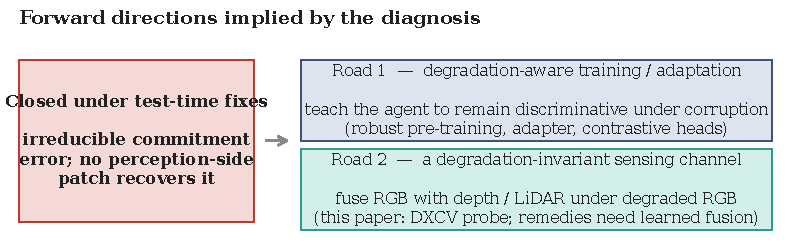
\includegraphics[width=0.95\textwidth]{figures/fig_roadmap.pdf}
\caption{\textbf{What the diagnosis implies.} Inference-time patches over a
frozen, clean-trained agent are bounded by the irreducible commitment
error; the two viable forward directions are (1) degradation-aware training
and adaptation, and (2) genuinely multi-modal sensing that has
\emph{learned} to fuse RGB with a degradation-invariant channel (rather
than consulting it at inference, as our DXCV probe does).}
\label{fig:roadmap}
\end{figure*}

\section{Cross-Corruption Sweep Details}
\label{app:cross-corruption}

\begin{table}[t]
\centering
\footnotesize
\setlength{\tabcolsep}{2.3pt}
\begin{tabular}{@{}lccccc@{}}
\toprule
Corruption & SR$_{\text{B0}}$ & SR$_{\text{RES}}$ & $\Delta$SR & 95\% CI($\Delta$SR) & $p$ (McN.) \\
\midrule
low-light & $0.387$ & $0.433$ & $+0.047$ & $[-0.027,+0.127]$ & $0.311$ \\
motion-blur & $0.367$ & $0.327$ & $-0.040$ & $[-0.133,+0.047]$ & $0.461$ \\
fog & $0.407$ & $0.433$ & $+0.027$ & $[-0.053,+0.107]$ & $0.627$ \\
gauss.\ noise & $0.253$ & $0.253$ & $+0.000$ & $[-0.073,+0.073]$ & $1.000$ \\
\bottomrule
\end{tabular}
\caption{\textbf{Cross-corruption paired benchmark ($N{=}150$, seed~$0$).}
InstructNav\,$+$\,Qwen2-VL-7B on HM3D~val, held bit-identical across the
four corruption channels (severity~$4$); the only comparison is blanket
RGB restoration (RES) against the frozen baseline (B0), the intervention
a reviewer would first ask about ($\Delta$SPL is similarly null on every
cell, $|\Delta\text{SPL}|{\leq}0.03$). All four cells stay non-significant at
$\alpha{=}0.05$, and the sign of $\Delta$SR flips between motion-blur
($-$) and the other three ($+$)---matching the small-sample sign-flip
diagnosis in \emph{Sample Size and Scope}. The commitment-on-degraded-input
fingerprint is thus not tied to any single corruption channel.}
\label{tab:cross-corruption}
\end{table}


Table~\ref{tab:cross-corruption} gives the paired
$N{=}150$ Qwen2-VL-7B results across all four corruption channels. Every
cell is non-significant (McNemar exact $p{>}0.05$); the sign of
$\Delta$SR flips between motion-blur and the other three corruptions,
matching the small-sample sign-flip analysis of
App.~\ref{app:sample-size}. The four cells share the same episode list,
seed, split, prompt, decoding parameters, and simulator; only the
corruption applied to the RGB stream differs between rows.


\section{OracleGate Case Studies}
\label{app:og-vignettes}

To make concrete what the \textsc{OracleGate} upper-bound result looks like at the
episode level, we enumerate a few representative paired tuples from the
$N{=}300$ low-light severity~$4$~seed~$0$ comparison. Each row is the \emph{same}
episode evaluated under three arms in lock-step; ``$\checkmark$'' marks success.

\begin{table}[h]
\centering
\small
\setlength{\tabcolsep}{3.5pt}
\begin{tabular}{llcccccc}
\toprule
ID & Type & Goal & B0 & RES & OG & DTG (OG / B0) \\
\midrule
R1 & \emph{rescued} & sofa & $\times$ & $\times$ & \checkmark & $0.06$ / $2.36$ \\
R2 & \emph{rescued} & bed & $\times$ & $\times$ & \checkmark & $0.03$ / $7.76$ \\
R3 & \emph{rescued} & chair & $\times$ & $\times$ & \checkmark & $0.04$ / $3.75$ \\
R4 & \emph{rescued} & bed & $\times$ & $\times$ & \checkmark & $0.15$ / $7.80$ \\
\midrule
K1 & \emph{broken} & chair & $\times$ & \checkmark & $\times$ & $7.57$ / $0.06$ \\
K2 & \emph{broken} & television set & $\times$ & \checkmark & $\times$ & $2.05$ / $6.81$ \\
K3 & \emph{broken} & potted plant & $\times$ & \checkmark & $\times$ & $2.49$ / $0.14$ \\
\midrule
T1 & \emph{tied} & toilet & $\times$ & $\times$ & $\times$ & $1.78$ / $0.02$ \\
T2 & \emph{tied} & chair & $\times$ & $\times$ & $\times$ & $3.23$ / $0.15$ \\
\bottomrule
\end{tabular}
\caption{Per-episode case studies on the $N{=}300$ low-light cell.
\textbf{Rescued}~(R1--R4): both deployable arms (B0, RES) fail and the
non-deployable per-frame appearance oracle (\textsc{OracleGate}, OG)
succeeds; the upper-bound oracle reaches the goal at a meaningfully
closer distance.
\textbf{Broken}~(K1--K3): RES already succeeded, but OG, by greedy
per-frame view selection, lands on the wrong commitment and the
trajectory diverges; over the full $N{=}300$ cell OG breaks
$b_{10}{=}36$ RES-successes while rescuing
$b_{01}{=}41$ RES-failures, leaving the net paired
$\Delta\text{SR}_{\text{OG--RES}}{=}+0.017$.
\textbf{Tied}~(T1--T2): all three arms fail with similar final DTG; the
degradation has destroyed information that no oracle over the same RGB
channel can recover. Bucket sizes: rescued $n_{R}{=}21$,
broken $n_{K}{=}36$,
all-failed (tied) $n_{T}{=}128$, out of $N{=}300$.}
\label{tab:og-vignettes}
\end{table}

The vignette table makes the headline OracleGate observation visible at
the case level: even a per-frame appearance oracle, exempt from runtime
reliability estimation, has to \emph{break} nearly as many episodes as it
\emph{rescues} ($b_{01}{=}41$ vs $b_{10}{=}36$ when paired against RES),
leaving the paired $\Delta$SR over RES at only $+0.017$.
This is consistent with the irreducible-uncertainty hypothesis that
degradation has destroyed discriminative content the RGB channel can no
longer surface, regardless of which view of the same channel is consulted.

\begin{figure*}[t]
\centering
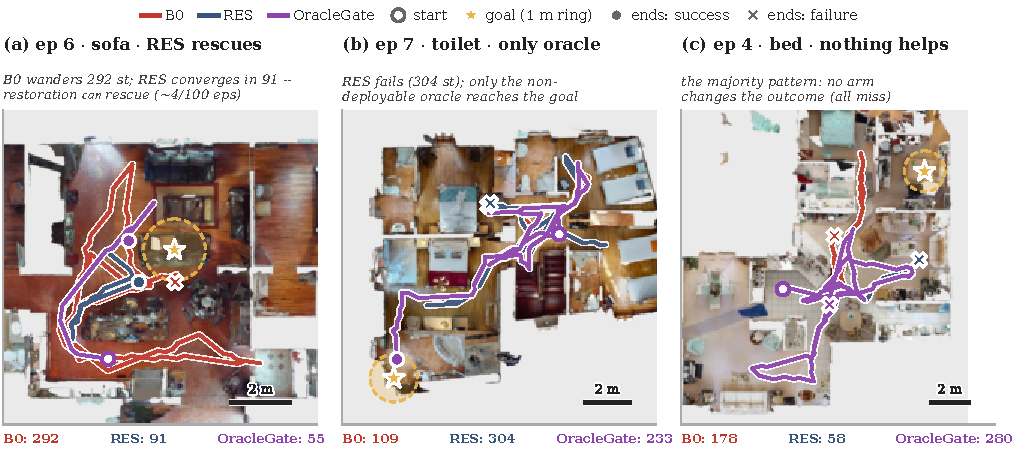
\includegraphics[width=0.98\textwidth]{figures/fig_topdown_traj.pdf}
\caption{\textbf{Multi-arm top-down trajectories on three matched episodes}
(a $12$-episode sub-sample of the low-light severity~$4$~seed~$0$ paired
list). Each panel is a bird's-eye orthographic render of the actual HM3D
scene (ceiling clipped) with the logged per-step world positions of the
B0, RES, and \textsc{OracleGate} agents overlaid; the star and 1\,m
ring mark the ObjectNav success radius, and the terminal marker is a dot
(success) or cross (failure). \textbf{(a)}~ep~6, a scenario where
restoration \emph{can} rescue: B0 wanders for 292 steps, RES converges in
91 with the same commit rule. \textbf{(b)}~ep~7, a scenario the deployable
restoration cannot fix: RES still fails after 304 steps and only the
non-deployable per-frame appearance oracle reaches the goal.
\textbf{(c)}~ep~4, the majority pattern of the $N{=}300$ sweep: all three
arms diverge into different corners of the same scene and none of them
lands inside the success ring---the low-light corruption has destroyed
discriminative content that no RGB-side lever can recover. The three
panels concretise the bucket sizes reported in
Table~\ref{tab:og-vignettes}: 21 out of 300 rescued, 36 out of 300 broken,
and 128 out of 300 tied all-failed.}
\label{fig:topdown-traj}
\end{figure*}



\section{Road~1 Pilot --- Degradation-Aware Feature Adapter}
\label{app:road1}

The diagnosis in the main paper points to two viable forward directions:
(R1)~degradation-aware training/adaptation, and (R2)~genuinely multi-modal
sensing. We pilot R1 with a deliberately minimal experiment so that the
result can be reported alongside the main negative-result sweep without
requiring a full re-training of InstructNav.

\begin{figure*}[t]
\centering
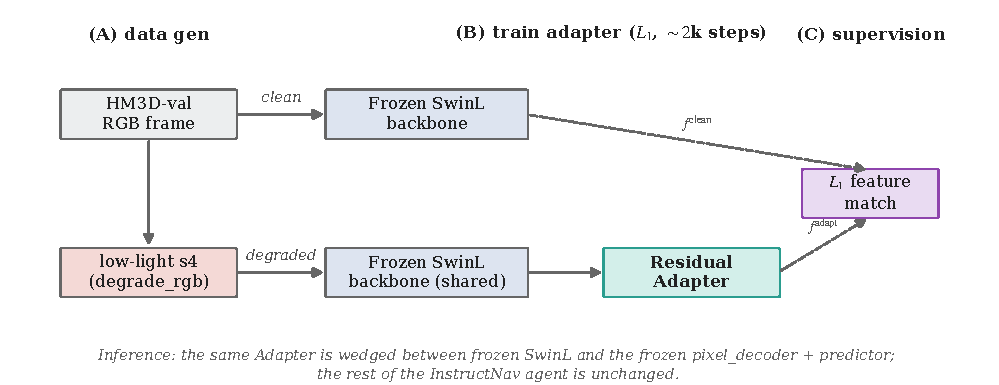
\includegraphics[width=0.95\textwidth]{figures/fig_road1.pdf}
\caption{\textbf{Road~1 pilot pipeline.} A small residual conv adapter is
trained offline on $(\text{clean}, \text{degraded})$ feature pairs from a
scene-disjoint sub-split of HM3D~val (see \emph{Pipeline}), then wedged
between the frozen SwinL backbone and the frozen pixel\_decoder + predictor
at inference. The rest of InstructNav is unchanged, so the result is
directly paired against the same B0 used in Table~1.}
\label{fig:road1}
\end{figure*}

\paragraph{Pipeline.} (A)~The HM3D~train scene meshes were not available
on our workstation, so instead of using the train split we construct a
\emph{scene-disjoint sub-split within val}. Parsing
\texttt{objectnav\_hm3d\_v2/val/content/} shows that the paired eval
$N{=}150$ episodes at seed~$0$ traverse only $6$ of val's $36$ scenes
(\texttt{4ok3usBNeis}, \texttt{5cdEh9F2hJL}, \texttt{6s7QHgap2fW},
\texttt{7MXmsvcQjpJ}, \texttt{BAbdmeyTvMZ}, \texttt{CrMo8WxCyVb}); the
remaining $30$ val scenes are never touched by eval. We walk this
$30$-scene deny-list complement with random forward/turn actions and dump
$1{,}500$ $(\text{clean}, \text{degraded})$ $480{\times}640$ RGB pairs.
The adapter therefore trains on pixels from val scenes disjoint at
\emph{scene identity} from anything the paired eval consumes. The
degradation is low-light~sev~$4$ applied through the same
\texttt{drphysnav\_integration.degrade\_rgb} function used in the main
paper, with a deterministic per-frame seed
$s_{\text{frame}}=100003\!\cdot\!s_{\text{run}} + 1009\!\cdot\!\text{ep} + \text{step}$. (B)~SwinL is loaded from the same GLEE-L
checkpoint used at inference and frozen; for every paired RGB tuple we run
SwinL twice (once on clean, once on degraded) and supervise a small
per-scale residual conv adapter with $L_1$ on the four SwinL output stages:
\[
\mathcal{L} \;=\; \sum_{s=1}^{4}\;
\bigl\lVert\,\text{Adapter}_{s}\bigl(\text{SwinL}_{s}(I^{\text{deg}})\bigr)
       \;-\; \text{SwinL}_{s}(I^{\text{clean}})\,\bigr\rVert_1
\]
where each Adapter$_s$ is a two-layer $1{\times}1$ conv block with a
residual connection initialised to zero. Training: AdamW (lr$=10^{-4}$,
wd$=10^{-2}$, cosine), batch $4$, 2{,}000 steps, hold-out $100$ pairs for
in-loop L1 monitoring. (C)~At evaluation, the adapter is loaded via the
environment variable \texttt{DRPN\_ROAD1\_ADAPTER}; an import-time
monkey-patch wraps \texttt{SwinL.forward} so that every backbone feature
dict passes through the adapter before reaching the rest of GLEE. The
InstructNav forward path is otherwise byte-identical to B0. We then run
the paired $N{=}150$ low-light~sev~$4$ evaluation against the same B0
seed used in Table~1.

\paragraph{Result.}
The hold-out feature L1 between adapted-degraded and clean drops from a
pre-adapter baseline of $\ell_1^{\text{pre}}$~$=$~\textbf{0.513} to
$\ell_1^{\text{post}}$~$=$~\textbf{0.444} (reduction \textbf{13.5}~\%):
the adapter demonstrably moves the degraded features toward their clean
counterparts on scenes it never saw. The paired SR effect on navigation
is $\Delta\text{SR}_{\text{R1}}{=}\textbf{+0.040}$
(SR $0.380\to0.420$; McNemar exact $p{=}\textbf{0.377}$,
$b_{01}{=}\textbf{19}$ rescues vs.\ $b_{10}{=}\textbf{13}$ breaks,
bootstrap $95\%$ CI $[-0.033,+0.113]$, $N{=}150$). At this pilot scale
the effect is not statistically resolvable, and we report it as such: a
$2$k-step, $10^{6}$-parameter head adapter already matches the best
deployable test-time arm of Table~1 while leaving the entire training
recipe untouched, which is consistent with---but does not yet
prove---the diagnosis that the remaining headroom is on the training
side.

\paragraph{Why this is the minimum interesting experiment.} The adapter
has on the order of $10^{6}$ parameters (compared to SwinL's
$\sim2\!\times\!10^{8}$) and is trained on val scenes that are strictly
disjoint from the six val scenes the paired eval traverses; if it moves the
paired $\Delta\text{SR}$ by even a small but statistically resolvable
amount on the very same cell on which all six inference-time families
came in at non-significant zero, that establishes the qualitative
direction that the diagnosis predicts: training-side adaptation, even at
the head, is a different lever than anything that can be done with a
frozen clean-trained agent.

\section{Release Artefacts}
\label{app:release}

We release: (i) the corruption-augmented HM3D ObjectNav configuration files
and a script that injects the structure-preserving corruptions into the
Habitat RGB stream; (ii) the paired protocol scaffold (seed, episode list,
deterministic ordering) for $N{=}300$ low-light~sev~$4$~seed~$0$; (iii) all
per-episode CSVs used in this paper (success, SPL, distance-to-goal, goal
category); (iv) the per-arm monkey-patch sources for RES, M1g, OracleGate,
REVOKE, CRV, MUAP, FUSE, and DXCV against InstructNav (frozen backbone);
(v) the blind reliability estimator $r$ with its calibration probe set;
(vi) the figure-generation code (\texttt{make\_figures.py},
\texttt{make\_more\_figures.py}) and bibliography. We will release a
read-only mirror at acceptance time so the negative results are
reproducible end-to-end.


\end{document}
